
\chapter[Estado del Arte]{Simulación de Materiales en Computación Gráfica: Estado del Arte}
\section{Introducción} %(hablar de los diferentes materiales, cómo los modelos "fáciles" no sirven)
El renderizado en computación gráfica es el intento de producir imágenes que representan una escena tridimensional, representada por medio de primitivas matemáticas como puntos, líneas, cubos, etc.

En los últimos años, el avance en el campo del renderizado de escenas ha sido muy notorio. El nivel de realismo presente en las imágenes obtenidas ha ido en aumento hasta el punto de ser de difícil distinción para un ser humano. Dichos avances han sido, en gran parte, debido al desarrollo de dispositivos de hardware gráficos más poderosos, ya que la teoría matemática que describe el comportamiento de la luz en escenas estuvo presente desde hace varias décadas \cite{Kajiya} mediante la denominada Ecuación del Rendering.


La ecuación es una aproximación, un modelo físico que intenta describir los aspectos considerados más importantes en el fenómeno de interacción de la luz con diversos objetos en una escena.

Lamentablemente, la ecuación es, en términos teóricos, no computable. Sin embargo, el estudio a lo largo de los años de técnicas que permitan aproximarla ha dado sus frutos y ha permitido la obtención de imágenes de un realismo asombroso.

A pesar de estos increíbles avances en un corto período de tiempo, el renderizado de una escena es un problema que involucra otros inconvenientes. El más notorio de ellos, es que la ecuación del rendering no tiene en cuenta qué {\em materiales} componen los objetos que definen la escena. En otras palabras, un objeto compuesto por madera no lucirá exactamente igual que uno compuesto por metales, ni por un material orgánico compuesto de tejidos. A la par del desarrollo de técnicas de iluminación global, han surgido técnicas que han intentado abordar materiales específicos \cite{} y familias de materiales \cite{}.

Estas técnicas buscan capturar la intrincada geometría propia de cada material. Diferentes estructuras microscópicas producen distintas apariencias, reflejando la luz de distinta manera, hecho que es interpretado por la percepción humana como diferentes materiales. Por ejemplo: una superficie metálica tiene un gran componente reflexivo, emitiendo luz en direcciones bien definidas, a diferencia de una superficie más opaca como un plástico. Dado que la ecuación del rendering usa los materiales como {\em caja negra}, los mismos deben ser modelados de una manera adecuada para ser integrados en las distintas técnicas de renderizado global.

Determinados materiales han recibido mayor atención debido a su ubicuidad en escenas de películas y video juegos, o a la facilidad de su diseño: agua, fuego, aire, humo, piel humana, madera, etc. Por esta razón, las imágenes sintéticas obtenidas presentan cierta asimetría en la calidad de los distintos materiales. En contraste, otros materiales han recibido menor atención, la cual puede atribuirse a una menor presencia en escenas o a una dificultad en el modelado y visualización, la cual ha resistido las técnicas más simples.

Entre estos materiales, aquellos sometidos a un proceso de cocción han permanecido entre los más dificultosos por su compleja geometría y los fenómenos lumínicos involucrados. Tal vez el caso más emblemático de los materiales cocidos es el pan, debido a su importancia en la vida cotidiana. Como nota de color, un reconocido  científico del área, Alain Fournier, pronunció en 2001 la frase "la Computación Gráfica todavía no ha sido capaz de renderizar de manera convincente una feta de pan". En las siguientes secciones mostraremos que unos pocos intentos por abordar el problema fueron realizados pocos años después.

\section{Modelos de Geometría de Materiales}
En esta sección presentaremos distintos modelos geométricos que han hecho su aparición a lo largo de los años en computación gráfica. Los mismos son el resultado de un balance entre detalle de representación, tiempos de cómputo y recursos de memoria utilizados.

\subsection{Modelos Procedimentales}
Un modelo procedimental resulta útil en determinadas situaciones donde la supervisión humana repetitiva no es adecuada.

Existen numerosos ejemplos donde se aplica una técnica de modelado procedimental.
En las siguientes sub-secciones presentaremos los casos más comunes de aplicación, los cuales constituyen estándares actuales en el modelado de dichos materiales.


\subsubsection{Plantas}
El modelado procedimental de plantas está basado en una interpretación de una tortuga que se mueve por un plano o el espacio, construyendo la geometría de los materiales \cite{Prusinkiewicz1986}.

Las gramáticas formales \cite{Chomsky1956} intentaron describir el lenguaje natural de forma matemática, donde sub-cadenas de caracteres son reemplazadas por otras.
Siguiendo esta idea, los sistemas-L \cite{Lindenmayer1968} pretenden realizar una descripción matemática de la geometría de las plantas.
El concepto central que permite entender el modelado procedimental utilizando sistemas-L es el de {\em reescritura}.
La reescritura consiste en una aplicación sucesiva de reglas que reemplazan determinadas partes en una descripción matemática por otras.
En un sistema-L, una cadena de caracteres representa la estructura de la planta.

\paragraph{Definición de sistema-L}
Sea $V$ un alfabeto (conjunto de caracteres), $V^{*}$ el conjunto de todas las palabras que se pueden formar con $V$ y $V^{+}$ el conjunto de todas las palabras que se pueden formar y no son vacías.
Una sistema-L de cadenas es una tripleta $G = (V,\omega,P)$, donde $V$ es el alfabeto, $\omega \in V^{+}$ es una cadena no vacía llamada {\em axioma} y $P \subset V \times V^{*}$ es un conjunto finito de reglas de producción.
Una producción $(a,\chi)$ se denota $a \rightarrow \chi$.
$a$ es llamado el {\em predecesor} y $\chi$ el {\em sucesor} de la producción.
Si no se especifica ninguna producción para $a$, se asume $a \rightarrow a \in P$.

Sea $\mu = a_{1}, \dots, a_{m}$ una palabra en $V$.
Se dice que la palabra $\mu_{1}, \dots, \mu_{m}$ es {\em derivada directamente} de $\mu$, y se nota $\mu \Rightarrow \eta$,  si y sólo si $a_{i} \rightarrow \mu_{i}, \forall i = 1, \dots, m$.

Una palabra $\eta$ es generada por $G$ si existe una secuencia de cadenas que conducen a $\eta$ desde el axioma, es decir, $\mu_{1},\dots,\mu_{n}$, de tal forma que $\mu_{1} = \omega$ y $\mu_{n} = \eta$ y $\mu_{1} \Rightarrow \dots  \Rightarrow \mu_{n}$.

Un ejemplo de esto es expuesto a continuación.
Si el axioma es $\omega = a$, y las reglas de producción son:
\begin{align*}
p1 &: a \rightarrow b,\\
p2 &: b \rightarrow ab,
\end{align*}

entonces una cadena de derivaciones podría resultar $a, b, ab, bb, abab, \dots$, donde las reglas aplicadas en cada paso serían $p1, p2, p1, p2$ (dos veces).

Estos sistemas fueron diseñados buscando representar las divisiones celulares existentes en ciertas amebas.
Sin embargo, luego se mostrará que los mismos pueden ser utilizados como modelos para capturar la geometría de diversos objetos.

\paragraph{Interpretación de Tortuga}
El estado de la tortuga se define por una tripleta $(x,y,\alpha)$, donde $x,y$ representan la posición de la tortuga y $\alpha$ es el ángulo hacia donde {\em apunta} la tortuga.
Dado un tamaño de paso $d$ y un incremento angular de $\delta$, la tortuga puede "programarse" para responder a cadenas de caracteres con la siguiente interpretación,

\begin{itemize}
\item F, moverse hacia adelante un paso d, dibujando,
\item f, moverse hacia adelante un paso d, sin dibujar,
\item +, rotar un ángulo $\delta$,
\item -, rotar un ángulo $-\delta$.
\end{itemize}

Al interpretarse el comando $F$, el nuevo estado de la tortuga será $(x',y',\alpha)$, donde $x' = x + d * cos(\alpha)$ y $y' = y + d * sin(\alpha)$. Se dibuja además una línea entre $(x,y)$ y $(x',y')$.
Al interpretarse el comando $f$ ocurre lo mismo, sólo que la línea no se dibuja.
Cuando se lee el comando $+$ (girar a la izquierda). el nuevo estado pasa a ser $(x,y,\alpha-\delta)$ y cuando se interpreta $-$ (girar a la derecha),  $(x,y,\alpha+\delta)$.

De esta forma, dada una cadena $\eta$, la interpretación de tortuga de la misma es la imagen que se genera al responder la tortuga a los comandos inducidos por $\eta$.
La Fig.~\ref{fg:tortuga} muestra un ejemplo de la figura resultante de la cadena FFF-FF-F-F+F+FF-F-FFF, donde la tortuga comienza {\em mirando} hacia arriba, y $\delta = 90^{\circ}$.

\begin{figure}
\center
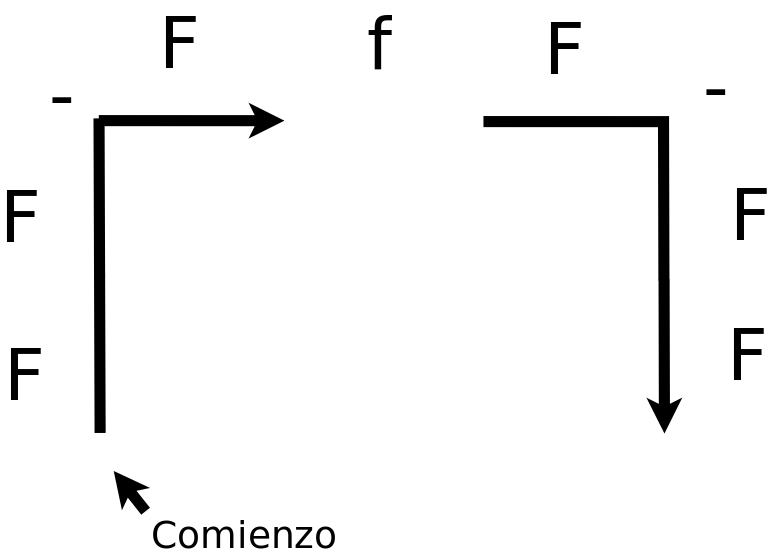
\includegraphics[width=8cm]{figures/tortuga}
\caption{Resultado de la interpretación de tortuga de una cadena de caracteres.}
\label{fg:tortuga}
\end{figure}

La Fig.~\ref{fg:tortuga} muestra otros ejemplos de sistemas-L, en los cuales se puede observar que con pocas reglas es posible obtener estructuras complejas y de gran belleza.

Usualmente, y debido a la utlización de recursión y repetición, estos sistemas dan lugar a figuras fractales, por lo cual se las utiliza para dibujar este tipo de estructuras autosimilares.

\begin{figure}
\center
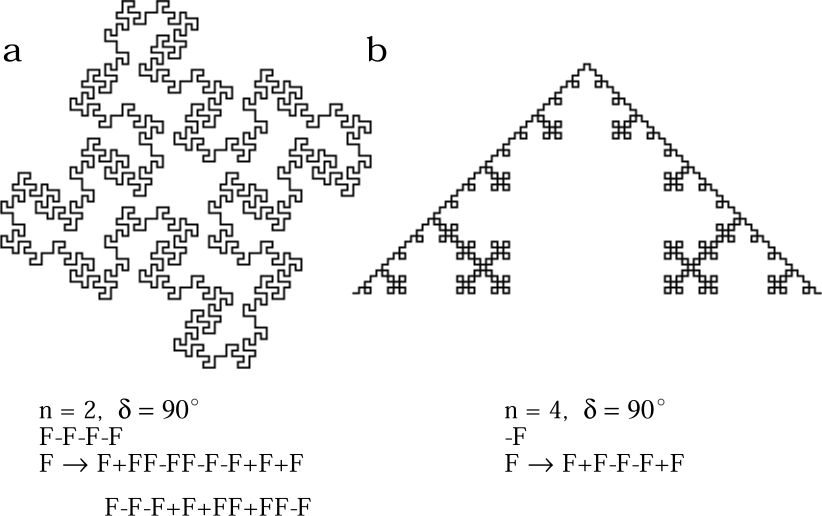
\includegraphics[width=13cm]{figures/sistemasL}
\caption{Sistemas-L generados utilizando distintos parámetros. $n$ es la cantidad de derivaciones utilizadas para producir la cadena que da origen a la figura. En (a), el axioma es F-F-F-F, mientras que en (b) es -F.}
\label{fg:sistemasL}
\end{figure}

Para lograr una imagen que semeje la estructura de árboles y plantas, es necesario introducir dos nuevos caracteres, los cuales son utilizados para generar estructuras ramificadas.
Utilizando una {\em pila} de estados, es posible alcanzar este comportamiento.
Los caracteres $[$, y $]$ se utilizan para mover el estado actual a la pila, y para reemplazar el estado actual con el de la pila, respectivamente.
El estado actual de la tortuga está representado por la tripleta antes mencionada.
Por lo tanto, al realizar la operación $]$, en general la posición y orientación de la tortuga cambiarán.
La utilización de un par $[\dots]$ produce que la tortuga dibuje una rama y vuelva al punto inicial, permitiendo continuar con la computación de otras partes de la estructura.

\begin{figure}
\center
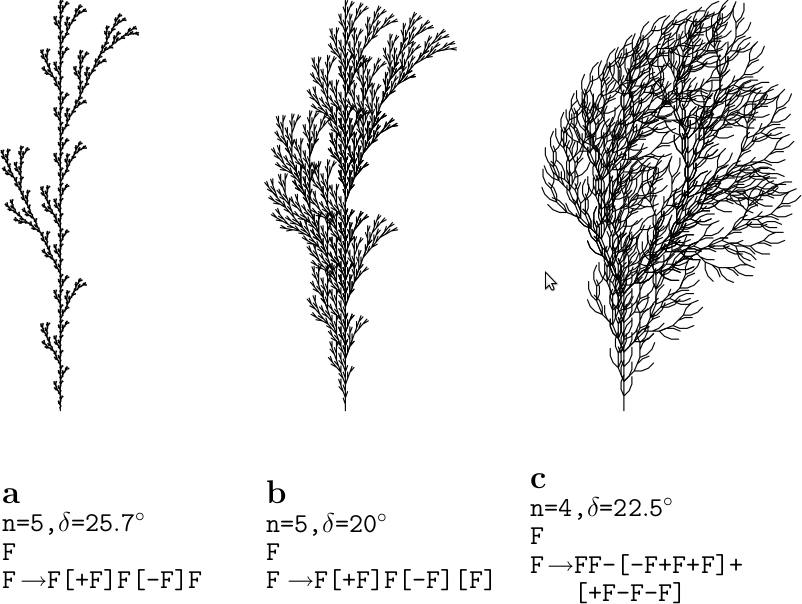
\includegraphics[width=13cm]{figures/sistemalcorchete}
\caption{Sistemas-L con pila de estados, utilizando distintos parámetros. Las imágenes muestran estructuras muy parecidas a plantas. $n$ es la cantidad de derivaciones utilizadas para producir la cadena que da origen a la figura.}
\label{fg:sistemasLcorchete}
\end{figure}


Existen numerosas variantes a estos sistemas, entre los cuales encontramos sistemas-L estocásticos, los cuales eligen reglas de reescritura de acuerdo a una probabilidad que se pasa como parámetro, sistemas-L paramétricos, los cuales hacen variar el ángulo y el paso a dibujar dependiendo de la posición de la cadena donde se encuentran, y muchos otros.
Además, el método es fácilmente generalizable en tres dimensiones, ver \cite{Prusinkiewicz1990} para obtener mayores detalles.

\subsubsection{Edificios y Ciudades}
Una de las ventajas del modelado procedimental es la capacidad de realizar el proceso prácticamente sin intervención humana, ahorrando costos y tiempos de diseño.
En esta línea se ubica el trabajo de \cite{Wonka2003}, donde un proceso automático genera, de manera casi instantánea, edificios arquitectónicamente coherentes, es decir, con ciertas características estructurales que deben ser respetadas.

La diferencia principal a la hora de utilizar sistemas-L para modelar edificios, es que los mismos no pueden ser modelados como una estructura que crece, sino que deben tratarse como conjuntos de objetos con una disposición específica.

Para lograr esto, en \cite{Wonka2003} se proponen varias definiciones, entre las que se encuentran gramáticas de división y gramáticas de control.

Una {\em forma} es un conjunto de líneas rectas en el espacio.
Las gramáticas de división seleccionan reglas para subdividir formas en formas más básicas (cubos, cilindros, etc.).


Una gramática puede ser definida de manera general como un álgebra de objetos $(U,+,-,F,\leq)$, cerrada bajo las operaciones $+$ y $-$, junto a un conjunto de operaciones $F$, de tal forma que si $u$ y $v$ son miembros de $U$, entonces $u+f(v)$ y $u-f(v)$ lo son, donde $f \in F$.
Una gramática $G=(N,T,R,I)$ es una tupla que consta de cuatro elementos, donde $N \subset U$ representa los nodos no terminales, $T \subset U$ los terminales, $I \subset N$ un conjunto de objetos iniciales y un conjunto de producciones $R \subseteq U \times U$.

%Para comprender mejor estos conceptos, definimos una gramática de conjuntos.
%Este tipo de gramáticas 

La Fig.~\ref{fg:splitgrammar} muestra un ejemplo del proceso involucrado en una gramática {\em de división}, en la cual una {\em forma} es dividida en otras, utilizando reglas definidas por dicha gramática, en este caso formando una secuencia de ventanas.
Como puede observarse, una gramática de este tipo divide de forma completa el espacio de las formas padre, en formas hijas de la misma.

Cuando el proceso llega a su fin, es decir, no existen nodos no terminales ($N$) en el desarrollo, entonces lo que se tiene es un {\em diseño} final.
La principal diferencia con los sistemas-L se basa en que en aquellos, las reescrituras no necesariamente ocupaban el mismo volumen, como sí debe ocurrir en estas gramáticas.

\begin{figure}
\center
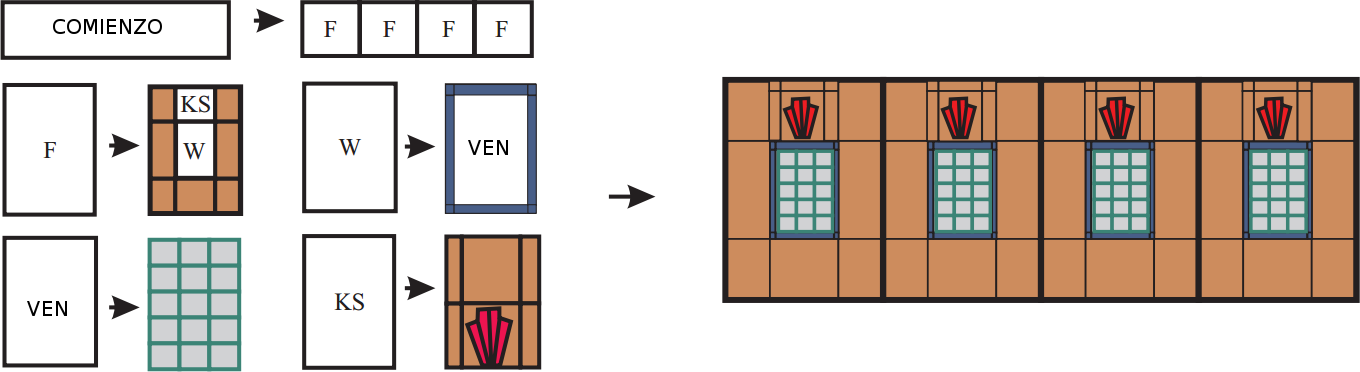
\includegraphics[width=13cm]{figures/splitgrammar}
\caption{Gramática de división mostrando los pasos seguidos para formar una secuencia de ventanas.}
\label{fg:splitgrammar}
\end{figure}

Por otro lado, las gramáticas de control permiten tomar decisiones de diferenciación sobre las divisiones, con la idea de generar al mismo tiempo aleatoriedad en los edificios resultantes.
Por ejemplo, se puede querer que la apariencia del primer piso de un edificio sea diferente al resto (puertas).
La Fig.~\ref{fg:controlgrammar} muestra un ejemplo de una gramática de control.

Las texturas, colores y otras decisiones pueden controlarse por medio de {\em atributos}.
Esto resulta útil para mantener la coherencia en un mismo piso, por ejemplo, o asegurar que todas las columnas del edificio seguirán un mismo diseño arquitectónico.
Los nodos terminales de la gramática presentan datos de posicionamiento con la forma $(c,a,v)$, donde $c$ es la posición en la división (fila, columna, capa, en $3D$), $a$ es el atributo y $v$ el valor que tomará.
Las gramáticas de control también cumplen el propósito de lograr una distribución correcta de las formas.
Por medio de ellas, es posible {\em excluir} elementos de ciertas posiciones indeseadas (por ejemplo una puerta en el tercer piso), utilizando los mismos atributos para elegir determinadas reglas por sobre otras, logrando coherencia y balance de formas en los resultados finales.

\begin{figure}
\center
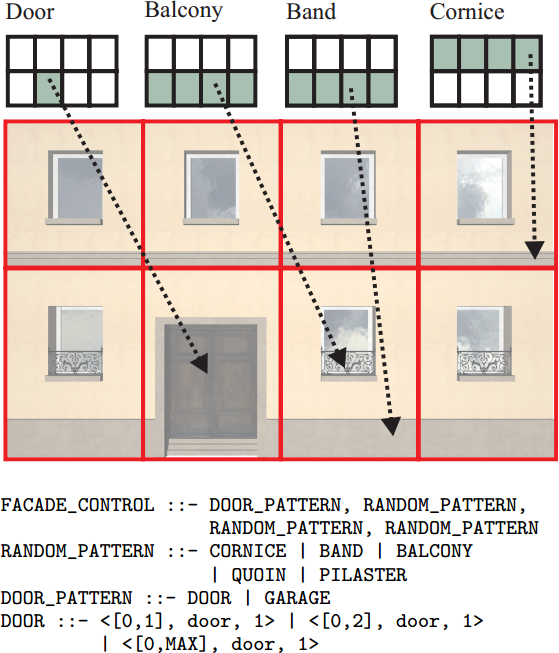
\includegraphics[width=11cm]{figures/controlgrammar}
\caption{Gramática de control.}
\label{fg:controlgrammar}
\end{figure}

La literatura de modelado procedimental de edificios y ciudades está creciendo en los últimos años \cite{Parish2001,Muller2006}.
La Fig.~\ref{edificios} muestra ejemplos de edificios generados procedimentalmente.



\begin{figure}
\center
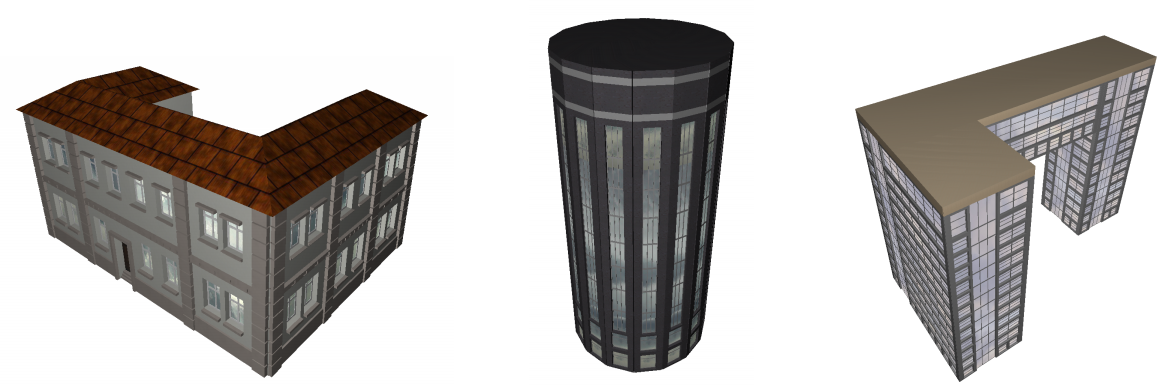
\includegraphics[width=11cm]{figures/edificios}
\caption{Edificios generados procedimentalmente por medio de gramáticas.}
\label{fg:edificios}
\end{figure}

\subsubsection{Fractales y Montañas}
Una forma particularmente interesante de modelar fenómenos de apariencia pseudo-aleatoria es a través de fractales \cite{Mandelbrot1982}.
Como en el caso de los sistemas-L, una única descripción matemática es lo suficientemente descriptiva como para encapsular todas los detalles, a diferentes escalas, de un fenómeno natural dado.
Esto resulta de particular interés en computación, donde los recursos de memoria no son infinitos.

En el siglo XIX, Brown describió el movimiento de partículas de polen en suspensión en agua, a lo cual se le otorgó el nombre de movimiento browniano.


%\subsubsection{Planetas}
\cite{Ebert2002}


\subsection{Modelos Físicos}
Desde el surgimiento del área, estos modelos han ido evolucionando gracias al incremento en el poder de cómputo del hardware gráfico disponible. Sin embargo, aún nos encontramos en los comienzos de una aplicación más difundida de los mismos.

\subsubsection{Fluídos}
Entre los primeros intentos por utilizar procesos físicos para modelar la apariencia de los materiales, encontramos ecuaciones que describen fluidos.
Las ecuaciones de Navier-Stokes describen un fluído cuya temperatura es prácticamente constante por medio de un campo de velocidades $\bold{u}$ y un campo de presiones $p$.
Dadas condiciones iniciales para $\bold{u}$ y $p$ cuando $t = 0$, la evolución de las cantidades puede describirse como sigue, independientemente del número de dimensiones,

\begin{align}
\nabla \cdot \bold{u} &= 0, \label{eq:eq1}\\
\frac{\partial \bold{u} }{\partial t} &= - (\bold{u} \cdot \nabla) \bold{u} - \frac{1}{\rho} \nabla p + \nu \nabla^{2} \bold{u} + \bold{f} \label{eq:eq2},
\end{align}

donde $\nu$ es la viscosidad cinemática del fluído, $\rho$ es la densidad y $\bold{f}$ es una fuerza externa.
Las ecuaciones modelan la conservación de masa (\ref{eq:eq1}) y de momento (\ref{eq:eq2}).

Además, deben tenerse en cuenta condiciones de borde.
Las mismas pueden variar en complejidad.
Por ejemplo, una implementación sencilla puede darse utilizando condiciones de borde periódicas, es decir, sin la existencia de {\em paredes} (el fluido se repite indefinidamente, este es el caso utilizado en el trabajo descripto aquí).
Un caso más complicado es una condición diferencial que describe el intercambio de masa con el ambiente.

Es posible combinar ambas ecuaciones para obtener una única ecuación de la velocidad.
Para esto, utilizaremos la descomposición Helmholtz-Hodge \cite{Chorin1990}, la cual establece que un campo vectorial $\bold{w}$ puede descomponerse como sigue, 

\begin{equation}
\label{eq:eq3}
\bold{w} = \bold{u} + \nabla q,
\end{equation}

donde $\bold{u}$ tiene divergencia $0$, es decir $\nabla\cdot\bold{u} = 0$.
Entonces, podemos definir un operador $\bold{P}$, el cual proyecta un campo vectorial $\bold{w}$ en su parte de divergencia $0$, $\bold{u} = \bold{P}\bold{w}$.
Dicho operador se puede definir implícitamente multiplicando $\nabla$ en ambos términos en la ecuación (\ref{eq:eq3}),

\begin{equation}
\label{eq:eq4}
\nabla\cdot\bold{w} = \nabla^{2} q.
\end{equation}

Una solución a esta ecuación está dada por

\begin{equation}
\label{eq:eq5}
\bold{u} = \bold{P}\bold{w} = \bold{w} - \nabla q,
\end{equation}

Si aplicamos el operador $\bold{P}$ en ambos lados de la ecuación (\ref{eq:eq2}), obtenemos una ecuación única para la velocidad,

\begin{equation}
\frac{\partial \bold{u} }{\partial t} = \bold{P} (- (\bold{u} \cdot \nabla) \bold{u} + \nu \nabla^{2} \bold{u} + \bold{f}) \label{eq:eq6},
\end{equation}

ya que $\bold{P}\bold{u} = \bold{u}$ y $\bold{P}\nabla p = 0$.
Esta ecuación es utilizada para derivar un algoritmo práctico para implementar apariencia de fluídos \cite{Stam1999}.
En la ecuación pueden verse un paso difusivo $\nu \nabla^{2} \bold{u}$, un paso de advección $- (\bold{u} \cdot \nabla) \bold{u}$ y una fuerza final aplicada $\bold{f}$.
Estos términos pueden resolverse por medio de la aplicación de métodos numéricos clásicos (por ejemplo diferencias finitas), por lo cual la solución final consiste en aplicar sucesivamente cada paso para obtener soluciones al campo vectorial $u$ en cada instante de tiempo $t$, finalmente proyectando el resultado con $P$.
El paso más complicado es el paso de proyección $P$, el cual se resuelve por medio de sistemas lineales, teniendo en cuenta que es un proceso de Poisson.

Cuando se conocen las velocidades $\bold{u}$, es posible aplicarlas a la utilización de partículas sobre el fluido, para proceder luego a su renderizado.

Este método se utiliza para modelar el comportamiento de agua y otros líquidos, además de algunos gases, nubes y humo, ver Figs.~\ref{fg:fluidos1},\ref{fg:fluidos2}.
La utilización de los procesos físicos subyacentes produce mayor realismo en el resultado que utilizar métodos heurísticos.
Desafortunadamente muchas veces esto resulta prohibitivo, no solo por costos computacionales, sino también por la complejidad en el diseño de los métodos, ya que se requiere muchas veces la participación de personas idóneas en la física utilizada.


\begin{figure}
\center
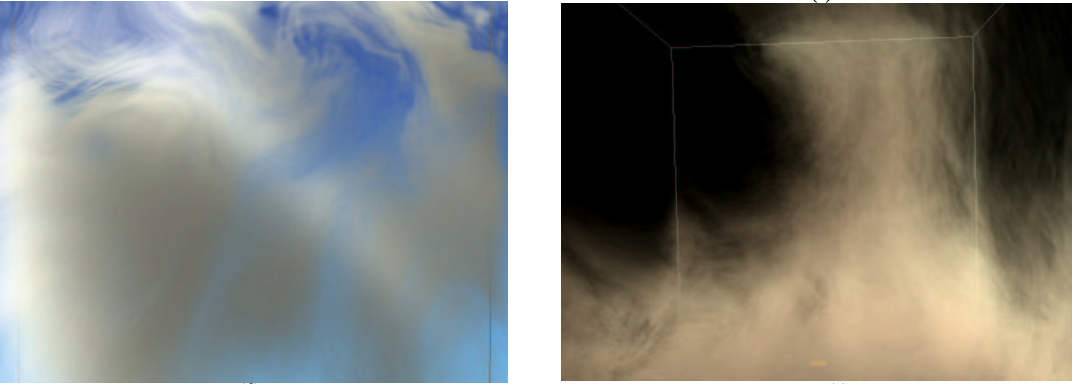
\includegraphics[width=11cm]{figures/fluidos1}
\caption{Nubes y humo generados utilizando métodos basados en las ecuaciones de Navier-Stokes.}
\label{fg:fluidos1}
\end{figure}

\begin{figure}
\center
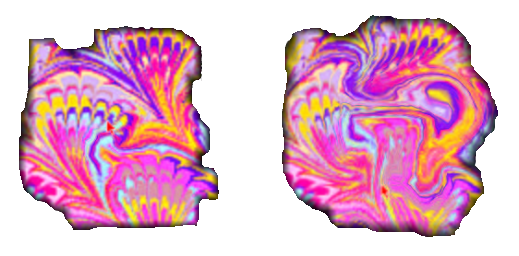
\includegraphics[width=11cm]{figures/fluidos2}
\caption{Fluidos generados utilizando métodos basados en las ecuaciones de Navier-Stokes.}
\label{fg:fluidos2}
\end{figure}

%\subsubsection{Telas}

\section{Representación Visual (Renderizado)}

Los materiales, además de presentar una geometría compleja, también presentan fenómenos particulares de interacción con la luz, los cuales incluyen translucencia, reflectancia, absorción, etc.
Debido a esto, en la década de $1980$ se simplificaron determinadas ecuaciones físicas para ser implementadas en computación gráfica, permitiendo modelar la apariencia de una gran variedad de materiales.

\subsection{Ecuación del Renderizado}

Esta ecuación modela el rebote de la luz en distintos tipos de superficie.

\begin{equation}
I(x,x') =  g(x,x')  \left[ \epsilon(x,x') + \int_{s}{\rho(x,x',x'')I(x,x'') dx''} \right],
\end{equation}
donde $I(x,x')$ es la intensidad de la luz que viaja de $x'$ a $x$ (sin oclusiones), $g(x,x')$ es un terminó geométrico que modela la oclusión que podría existir entre $x$ y $x'$, $\epsilon(x,x')$ es la intensidad de la luz emitida desde $x'$ a $x$, $\rho(x,x',x'')$ es la intensidad de la luz emitida de $x''$ a $x$ por medio de una superficie en $x'$ (esta cantidad será llamada BRDF en una sección posterior), y $S=\bigcup{s_{i}}$ es la unión de todas las superficies de la escena.
De esta forma, $x$,$x'$ y $x''$ varían sobre todas las superficies de la escena.
La ecuación es una aproximación a la ecuación del electromagnetismo de Maxwell, pero sólo tiene en cuenta fenómenos óptico-geométricos.
Además existe una superficie $S_{0}$, la cual es un semi-hemisferio que engloba a toda la escena.
$I(x,x')$ significa la radiación de energía por unidad de tiempo por unidad de superficie de destino por unidad de superficie de origen ($joule/m^{4} s$).
El término geométrico se hace $0$ si los puntos en consideración no son mutuamente visibles.

Por medio del modelado de cada término de forma separada, es posible obtener una gran cantidad de superficies.
Trabajos previos a la aparición de la ecuación del renderizado habían logrado resultados parciales, sin saber que una única ecuación podía englobar todos los fenómenos en investigación hasta ese entonces.
Como resultado de este modelo, hoy es posible llamar a los métodos previos a este como especializaciones o casos particulares de la ecuación del renderizado.

Fuera de la ecuación quedan efectos más complejos, como la difracción y la polarización.
De esta forma, la ecuación modela el comportamiento de la luz entre las superficies de la escena.
Más detalles de la misma pueden ser consultados en \cite{Kajiya1986}.

Si lo que se pretende modelar son fenómenos volumétricos, entonces debe atenderse a ciertas generalizaciones de la ecuación, como se ve en la siguiente sub-sección.

\subsection{Ecuación del Renderizado de Volúmenes}

Esta ecuación representa el comportamiento de la luz en volúmenes.

\begin{equation}
(\vec{\omega} \cdot \nabla) = - \sigma_{a}(\bold{x}) L(x \rightarrow \vec{\omega}) - \sigma_{s}(\bold{x}) L(x \rightarrow \vec{\omega}) + \sigma_{a}(\bold{x}) L_{e}(x \rightarrow \vec{\omega}) + \sigma_{s}(\bold{x}_{t}) L_{i}(x \rightarrow \vec{\omega})
\end{equation}

Podemos expresar esta ecuación en forma integral integrando ambos lados de la igualdad, obteniendo,

\begin{equation}
\begin{aligned}
L(x \leftarrow \vec{\omega}) = T_{r}(\bold{x} \leftrightarrow \bold{x_{s}}) L(\bold{x_{s}} \rightarrow -\vec{\omega}) + \\
\int_{0}^{s}{T_{r}(\bold{x} \leftrightarrow \bold{x_{t}}) \sigma_{a}(\bold{x}) L_{e}(x \rightarrow -\vec{\omega}) dt } + \\
\int_{0}^{s}{T_{r}(\bold{x} \leftrightarrow \bold{x_{t}}) \sigma_{a}(\bold{x_{t}}) L_{i}(x_{t} \rightarrow -\vec{\omega})  }
\end{aligned}
\end{equation}



\subsection{BRDFs}
\subsection{Radiancia}
\subsection{Simplificaciones}
Todas estas simplificaciones son realizadas a escala humana, es decir, sin tener en consideración la naturaleza microscópica de la luz. En esta escala, las trayectorias que describe la luz son aproximadas por líneas rectas.
\subsubsection{Ray Tracing}
\subsubsection{Radiosity}
\subsubsection{Photon Mapping}
\subsubsection{Ray Marching}
\subsubsection{Volume Rendering}

\section{Materiales específicos:}
\subsection{Agua}
\subsection{Fuego}
\subsection{Humo}
\subsection{Piel}
\subsection{Otros}


\section{Conclusiones}

